\chapter{Entwicklung des Testsystems}
\label{ch:model}

Um die in \cref{ch:caseStudy} beschriebene Fallstudie durchführen zu können, wurde zunächst TestingHadoop mithilfe des \gls{ss}"=Frameworks entwickelt.
Das Testsystem bildet \uA vereinfacht die für die Fallstudie relevanten YARN"=Komponenten ab und besteht aus den drei im Folgenden beschriebenen, architektonischen Schichten.

Da für die in \cite{Eberhardinger2018} durchgeführte Fallstudie das in diesem Kapitel beschriebene System genutzt wurde, wurden entsprechende Teile der Beiträge dieses Kapitels dort bereits publiziert.

\section{Grundlegende Architektur des Testmodells}
\label{sec:modelArchitecture}

Um Hadoop mit der Selfbalancing"=Komponente mit den in \cref{sec:requirements} beschriebenen Anforderungen prüfen zu können, wird mithilfe des \ac{ss}"=Frameworks ein vereinfachtes Modell der relevanten \ac{YARN}"=Komponenten entwickelt.
Dieses \ac{YARN}"=Modell wird mithilfe des Treibers mit dem realen Cluster verbunden.
Daraus resultiert folgende Drei"=Schichten"=Architektur für das gesamte Testmodell:

\begin{figure}[h]
    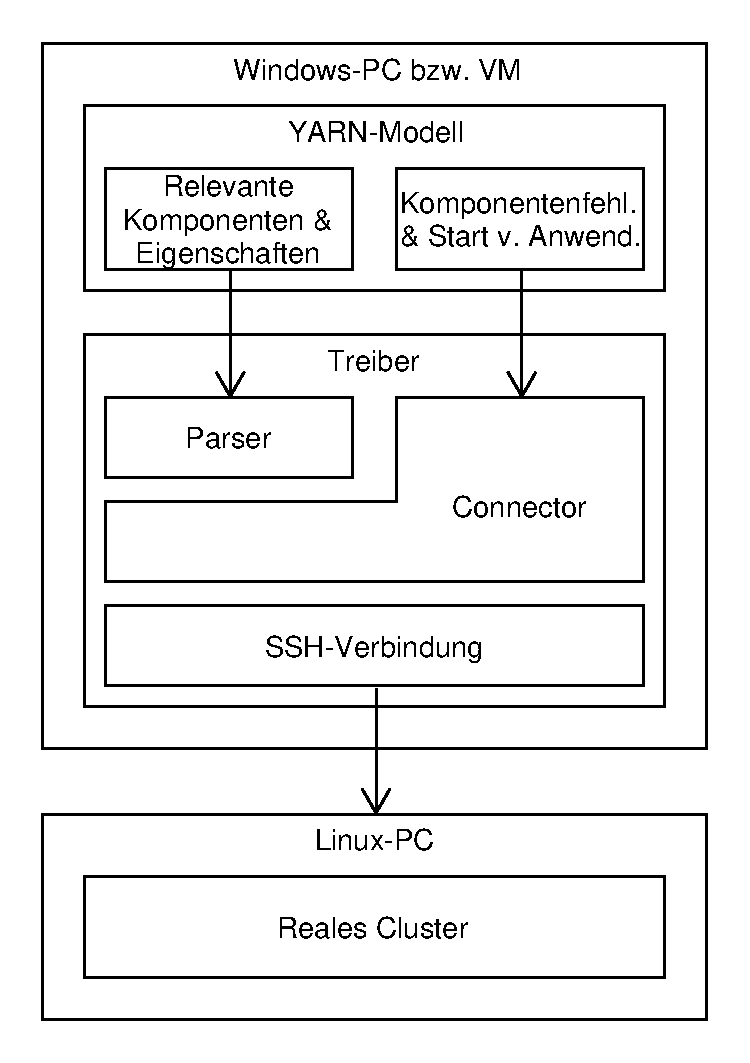
\includegraphics[width=0.6\columnwidth]{./images/modelArchitecture.pdf}
    \caption{Grundlegende Architektur des Testsystems}
    \label{fig:modelArchitecture}
\end{figure}

Das \ac{YARN}"=Modell stellt die oberste Schicht des Testmodells dar.
Es bildet das Kernstück dieser Fallstudie, da dieses Modell mit den hierin abgebildeten, für diese Fallstudie relevanten \ac{YARN}"=Komponenten und implementierten Komponentenfehlern, dem Controller und dem Oracle direkt im Rahmen des modellbasierten Testens mit \ac{ss} interagiert.
Folgende Komponenten sind im \ac{YARN}"=Modell enthalten:

\begin{description}
    \item [Controller] \hfill \\
        Steuert den Ablauf einer Testausführung und das Zusammenspiel zwischen den Komponenten des \ac{YARN}"=Modells.
    \item [Relevante \ac{YARN}"=Komponenten und Eigenschaften] \hfill \\
        Bilden die grundlegende Architektur von Hadoop \ac{YARN} ab.
        Implementiert wurden in dieser Fallstudie die Nodes, Anwendungen, Attempts und Container mit den jeweils relevanten Eigenschaften zur Durchführung der Fallstudie.
    \item [Komponentenfehler der \ac{YARN}"=Komponenten] \hfill \\
        Bilden die bei den Tests zu injizierenden Komponentenfehler der jeweiligen \ac{YARN}"=Komponenten.
    \item [Oracle] \hfill \\
        Validiert die in Form von Constraints in den jeweiligen \ac{YARN}"=Komponenten implementierten Anforderungen.
    \item [Client] \hfill \\
        Dient zum starten und beenden von Benchmarks im Cluster.
    \item [Benchmark"=Controller] \hfill \\
        Enthält das Transitionssystem zur Auswahl der Benchmarks und steuert diese.
\end{description}

Die Verbindung zwischen dem \ac{YARN}"=Modell und dem realem Cluster bildet der Treiber.
Er besteht aus folgenden Komponenten:

\begin{description}
    \item [Parser] \hfill \\
        Verarbeitet die Monitoring"=Ausgaben vom realen Cluster und konvertiert diese für die Nutzung im \ac{YARN}"=Modell.
    \item [Connector] \hfill \\
        Abstrahiert die Verbindung zum realen Cluster und die dabei auszuführenden Befehle.
    \item [SSH"=Verbindung]  \hfill \\
        Stellt die Verbindung zum realen Cluster her.
\end{description}

Der Parser wird hierbei nur zur Durchführung des Monitoring benötigt und nutzt wiederum den Connector zum abrufen der Daten.
Andere Befehle und Zugriffe auf das reale Cluster, wie \zB das Injizieren von Komponentenfehlern, werden direkt mithilfe des Connectors durchgeführt.

Die Implementierung des \ac{YARN}"=Modells wird in \cref{sec:yarnModel} beschrieben, die Implementierung des Treibers in \cref{sec:sshDriver}.
Die Umsetzung des realen Clusters wird in \cref{sec:realCluster} beschrieben.


\section{Implementierung des \acs{YARN}"=Modells}
\label{sec:yarnModel}

Das implementierte \ac{YARN}"=Modell besteht, wie bereits in \cref{sec:modelArchitecture} gezeigt, aus fünf Komponenten und den Komponentenfehlern der hier relevanten \ac{YARN}"=Komponenten.
Die vier implementierten \ac{YARN}"=Komponenten sind die Anwendungen, ihre Attempts und Container, sowie die Nodes.
Zudem wurde eine Klasse implementiert, die zur Repräsentation des \ac{RM} dient, und als Controller im Rahmen des Testens mit \ac{ss} dient.
Einen Überblick über den Aufbau des implementierten \ac{YARN}"=Modells gibt folgendes Klassendiagramm:

\begin{figure}[h]
    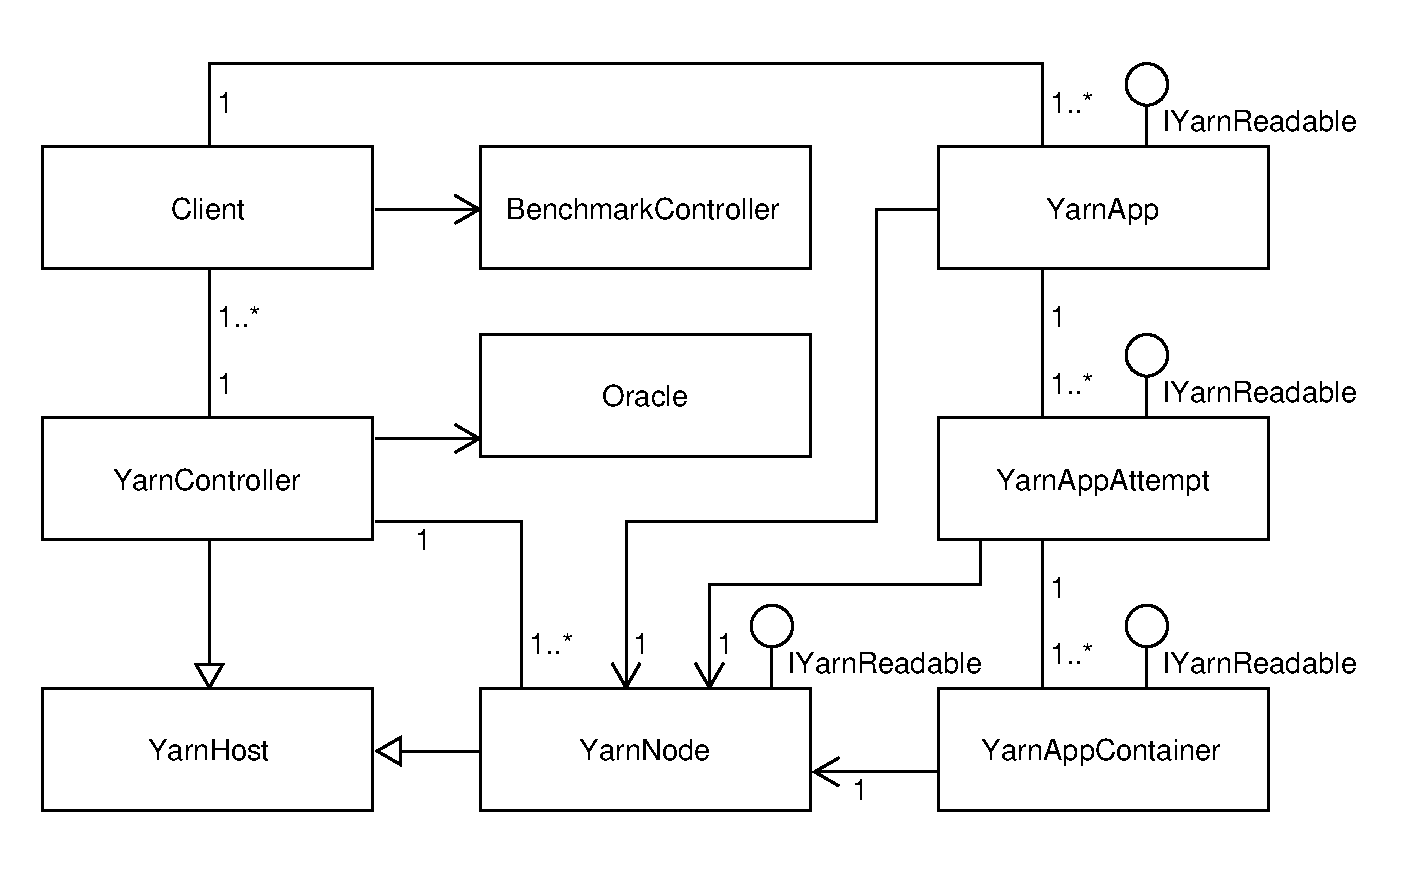
\includegraphics{./resources/yarnModel_ls_MA.pdf}
    \caption[Grundlegender Aufbau des \acs{YARN}"=Modells]
        {Grundlegender Aufbau des \acs{YARN}"=Modells.
        Assoziationen und weitere Verbindungen zum Treiber und \acs{ss} sind hier aus Gründen der Übersichtlichkeit nicht dargestellt.}
    \label{fig:yarnModelClassDiagram}
\end{figure}

Im Klassendiagramm wird zudem ersichtlich, dass jedem Client mehrere Anwendungen in Form der Klasse \texttt{YarnApp} zugeordnet sind, jeder Anwendung mehrere Attempts (\texttt{YarnAppAttempt}) und jedem Attempt mehrere Anwendungs"=Container (\texttt{YarnAppContainer}).
Der Client stellt somit auch die den relevanten \ac{YARN}"=Komponenten übergeordnete Komponente dar.

Zunächst wird im Folgenden zunächst die dem Modell übergeordnete zentrale Klasse \texttt{Model} erläutert, danach die relevanten \ac{YARN}"=Komponenten mit ihren Komponentenfehlern, anschließend die anderen Komponenten des \ac{YARN}"=Modells.

\subsection{Die Klasse Model}
\label{sec:modelClass}

Die Klasse \texttt{Model} stellt die zentrale Schnittstelle des Testsystems mit \ac{ss} dar.
Da diese Klasse auch das gesamte Modell repräsentiert, wird sie zur Verwaltung des von \ac{ss} auszuführenden Modells genutzt.
Hierfür werden alle Komponenten wie Clients oder Anwendungen zusätzlich zur Struktur innerhalb des Modells auch direkt in entsprechenden Eigenschaften dieser Klasse gespeichert, welche zur Interaktion mit \ac{ss} entsprechend markiert sind (vgl. \cref{subsec:ssharpModel}).

Daneben dient die Klasse auch zur Initialisierung des gesamten Modells.
Hierbei werden zunächst der Controller, der Treiber in Form der benötigten Parser und Connectoren, sowie die Nodes des Clusters initialisiert.
Anschließend wird für jeden Client eine gewisse Anzahl an \texttt{YarnApp}"=Instanzen zum Speichern der Daten von Anwendungen, für jede Anwendung eine gewisse Anzahl an \texttt{YarnAppAttempt}"=Instanzen für Attempts, sowie für jeden Attempt eine gewisse Anzahl an \texttt{YarnAppContainer} für die Daten der Anwendungs"=Container initialisiert.
Die genaue Anzahl der erzeugten Instanzen kann hierbei für jede \ac{YARN}"=Komponente und auch für Clients nach Bedarf angepasst werden, wodurch auch einzelne Komponenten wie \zB in der Fallstudie die Anwendungs"=Container, deaktiviert werden können.

\subsection{Relevante \acs{YARN}"=Komponenten}
\label{sec:yarnComponents}

Die vier implementierten, relevanten \ac{YARN}"=Komponenten sind die Anwendungen, ihre Attempts und Container sowie die Nodes des Clusters.
Obwohl die die Anwendungs"=Container in dieser Fallstudie nicht benötigt werden, waren sie für die in \cite{Eberhardinger2018} beschriebene Fallstudie notwendig, welche ebenfalls mit dem hier beschriebenen Modell durchgeführt wurden.

\subsubsection{Übersicht der implementierten Komponenten}
\label{subsec:yarnComponentsOverview}

Eine Übersicht über die Implementierung der \ac{YARN}"=Komponenten gibt folgendes Klassendiagramm:

\begin{figure}[h]
    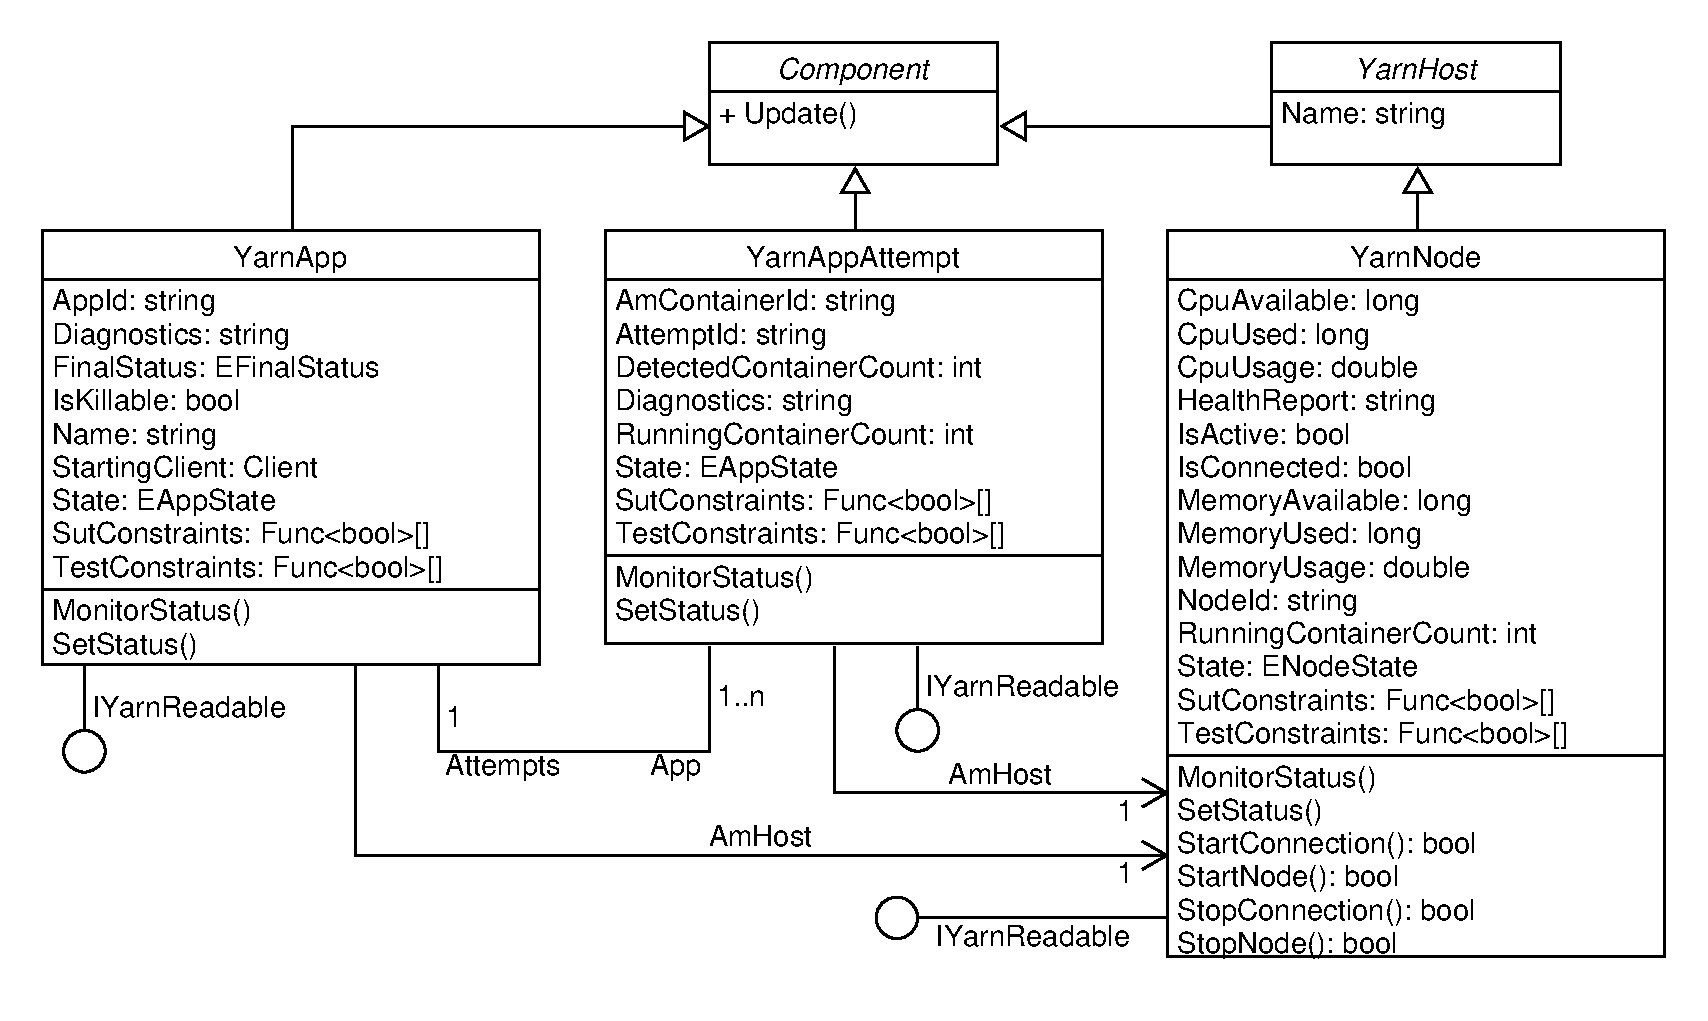
\includegraphics[width=\columnwidth]{./resources/yarnComponents.pdf}
    \caption[Für die Fallstudie relevante, implementierte \acs{YARN}"=Komponenten mit den wichtigsten Eigenschaften und Methoden]
        {Für die Fallstudie relevante, implementierte \acs{YARN}"=Komponenten mit den wichtigsten Eigenschaften und Methoden.
        Dies sind alle für die spätere Durchführung und zur Ausgabe des Zustandes (vgl. \cref{subsec:dataOrganisation}) wichtigen Eigenschaften und Methoden.
        Aus Gründen der Übersichtlichkeit sind die implementierten Komponentenfehler, einige der \texttt{IYarnReadable} bereitgestellten, relevanten Eigenschaften und Methoden, sowie die Klasse \texttt{YarnAppContainer} nicht aufgeführt.}
    \label{fig:yarnComponentsClassDiagram}
\end{figure}

Die Eigenschaft \texttt{AmHost} speichert den ausführenden Node des \ac{AppMstr} der Anwendung bzw. des Attempts, die Eigenschaft \texttt{IsKillable} gibt an, ob eine Anwendung derzeit ausgeführt ist und somit vorzeitig abgebrochen werden kann.
Die Eigenschaften \texttt{Diagnostics} bzw. \texttt{HealthReport} stellen von Hadoop zur Verfügung gestellte weitere Informationen bei Fehlern dar.
Die \texttt{State}"=Eigenschaften bzw. \texttt{FinalState} speichern die von Hadoop angegebenen Zustände der \ac{YARN}"=Komponenten.
Hierfür wurden entsprechende Auflistungen basierend auf den in \cite{HadoopRmApi271} angegebenen möglichen Werten für die jeweiligen Zustände im Modell implementiert.

Da für diese Fallstudie die Daten der Container selbst nicht relevant sind, wird im hier verwendeten Modell nur gespeichert, wie viele Anwendungs"=Container beim Monitoring im aktuellen Testfall (\texttt{RunningContainerCount}) bzw. für alle bisher ausgeführten Testfälle kumuliert (\texttt{DetectedContainerCount}) erkannt wurden.
Für die Tests in \cite{Eberhardinger2018} werden die Daten der Container genauso wie die der anderen \ac{YARN}"=Komponenten gespeichert.
Hierfür enthalten die Klassen \texttt{YarnAppAttempt} und \texttt{YarnAppContainer} entsprechende Eigenschaften zur jeweiligen Zuordnung analog zu denen zwischen \texttt{YarnApp} und \texttt{YarnAppAttempt}.
Analoge Zuordnungen bestehen auch zu den Clients bzw. den Anwendungs"=Containern, sofern benötigtt.
Die Eigenschaft \texttt{AmContainerId} speichert zudem die Container"=ID des \ac{AppMstr}"=Containers.

Die Eigenschaften mit dem Präfix \texttt{CPU} bzw. \texttt{Memory} in \texttt{YarnNode} dienen zur Speicherung der derzeitigen Auslastung der CPU"=Kerne bzw. des Speichers eines Nodes.
Benötigt werden diese Werte zur in \cref{subsubsec:simulationFaultActivation} beschriebenen Berechnung, ob ein Komponentenfehler aktiviert oder deaktiviert wird.

Die Eigenschaften \texttt{SutConstraints} und \texttt{TestConstraints} sowie die Methoden \texttt{MonitorStatus()} und \texttt{SetStatus()} werden von \texttt{IYarnReadable} bereitgestellt und speichern die Constraints bzw. dienen zur Durchführung des Monitorings der implementierten Komponenten.
Die Start"= und Stop"=Methoden sowie die Eigenschaften \texttt{IsActive} und \texttt{IsConnected} in \texttt{YarnNode} dienen zur Identifikation und Injizierung bzw. Reparieren der Komponentenfehlern.
Diese Eigenschaften und Methoden werden daher auf den folgenden Seiten näher beschrieben.

Neben den dargestellten, relevanten Eigenschaften und Methoden wurden zahlreiche weitere implementiert, welche einerseits zur Vollständigkeit der implementierten Komponenten für die Tests in \cite{Eberhardinger2018}, andererseits auch zur Ausführung mithilfe des \ac{ss}"=Frameworks benötigt werden.
Letztere sind \zB zur Speicherung von Strings notwendig, welche aufgrund der Einschränkungen von \ac{ss} (vgl. \cref{sec:ssharp}) nicht jederzeit frei genutzt werden können.
Strings sind im \ac{YARN}"=Modell daher zur Speicherung immer als  \texttt{char}"=Arrays implementiert, werden jedoch zur einfacheren Nutzung im Modell in Strings konvertiert:

\begin{lstlisting}[label=lst:modelCharArrayAsString,style=cs,
caption={[Implementierung der Eigenschaft AppId]
    Implementierung der Eigenschaft \texttt{AppId}.
    Die beiden Methoden \texttt{GetCharArrayAsString} und \texttt{SetCharArrayOnString} führen die Konvertierung in den \texttt{char}"=Array bzw. des \texttt{char}"=Arrays in einen String durch.}]
public char[] AppIdActual { get; }

[NonSerializable]
public string AppId
{
  get { return ModelUtilities.GetCharArrayAsString(AppIdActual); }
  set { ModelUtilities.SetCharArrayOnString(AppIdActual, value); }
}
\end{lstlisting}

Die \texttt{Update()}"=Methoden starten bei allen vier implementierten \ac{YARN}"=Komponenten die jeweiligen Monitoring"=Funktionen, bei \texttt{YarnNode} werden zudem \texttt{StartNode()} und \texttt{StartConnection()} ausgeführt um mögliche zuvor injizierte Komponentenfehler im realen Cluster zu reparieren.

Da bei der Ausführung des Modells durch \ac{ss} keine neuen Instanzen erzeugt werden können (vgl. \cref{sec:ssharp}), dienen die jeweiligen IDs der Komponenten auch als Indikator, ob die jeweilige Komponenten"=Instanz derzeit benötigt wird und somit Daten gespeichert werden sollen.
Daher wird das Monitoring auch nur dann ausgeführt, wenn der Instanz eine nicht leere ID \zB in Form der \texttt{AppId} zugewiesen wurde.

\subsubsection{Implementierung der Komponentenfehler}
\label{subsubsec:yarnComponentFaults}

Die im \ac{YARN}"=Modell implementierten Komponentenfehler wurden direkt in den entsprechenden \ac{YARN}"=Komponenten implementiert.
Implementiert wurden hierbei mit \texttt{NodeDeadFault} und \texttt{NodeConnectionErrorFault} zwei jeweils als \texttt{TransientFault} definierte Komponentenfehler für die durch \texttt{YarnNode} repräsentierten Nodes.
Während durch \texttt{NodeDeadFault} der komplette Node beendet wird, trennt \texttt{NodeConnectionErrorFault} nur die Verbindung des Nodes zum Cluster.
Die dazugehörigen Effekt"=Klassen der Komponentenfehler sind jeweils als innere Klassen in \texttt{YarnNode} implementiert.

Die Injizierung und das Reparieren der beiden Fehler geschieht mithilfe der vier Stop- bzw. Start"=Methoden wie \zB \texttt{StopNode()}, die bereits im Klassendiagramm in \cref{fig:yarnComponentsClassDiagram} zu sehen sind.
Wenn ein Komponentenfehler durch das Framework aktiviert wird, wird durch die Effekt"=Klasse die jeweilige Stop"=Methode aufgerufen und so der Fehler injiziert:

\begin{lstlisting}[label=lst:faultInjection,,style=cs,
caption={[Injizierung des Komponentenfehlers NodeDeadFault]
    Injizierung des Komponentenfehlers \texttt{NodeDeadFault} (gekürzt).
    Sollte der Node nicht beendet werden, wird die Injizierung einmalig erneut versucht.
    \texttt{CmdConnector.Faulting} stellt die zur Injizierung verwendete SSH"=Verbindung dar.}]
public class YarnNode : YarnHost, IYarnReadable
{
  [NodeFault]
  public readonly Fault NodeDeadFault = new TransientFault();
  public IHadoopConnector FaultConnector { get; set; }
  
  public bool StopNode(bool retry = true)
  {
    if(IsActive)
    {
      var isStopped = FaultConnector.StopNode(Name);
      if(isStopped)
        IsActive = false;
      else if(retry)
        StopNode(false); // try again once
    }
    return !IsActive;
  }
  
  [FaultEffect(Fault = nameof(NodeDeadFault))]
  public class NodeDeadEffect : YarnNode
  {
    public override void Update()
    {
      StopNode();
    }
  }
}

public class CmdConnector : IHadoopConnector
{
  private SshConnection Faulting { get; }
  
  public bool StopNode(string nodeName)
  {
    var id = DriverUtilities.ParseInt(nodeName);
    Faulting.Run($"{Model.HadoopSetupScript} hadoop stop {id}", IsConsoleOut);
    return !CheckNodeRunning(id);
  }
}
\end{lstlisting}

Das Reparieren von Komponentenfehlern geschieht analog hierzu.
Hierfür werden in der \texttt{Update()}"=Methode die beiden Start"=Methoden aufgerufen, die einen Fehlerhaften Node reparieren.
Eine Besonderheit bildet hierbei die Reparatur des Komponentenfehlers \texttt{NodeConnectionErrorFault}, bei der der Node komplett neu gestartet wird, da es sonst passieren kann, dass der wieder ans Netzwerk angebundene Node sich nicht mit dem \ac{RM} verbindet.

Ob ein Komponentenfehler in einem Testfall aktiviert wird, entscheidet sich anhand der Auslastung des Nodes.
Hierfür sind beide Komponentenfehler mit dem Attribut \texttt{NodeFault} versehen, mit dessen Hilfe entschieden wird, ob ein Komponentenfehler aktiviert oder deaktiviert und somit injiziert bzw. repariert wird.
Der Entscheidungsprozess hierfür ist in \cref{subsubsec:simulationFaultActivation} beschrieben.

Da beide Fehler zudem auch gleichzeitig aktiviert werden können, wurde \texttt{NodeDead""Fault} mithilfe entsprechender \ac{ss}"=Funktionen eine höhere Priorität vergeben, wodurch dieser Vorrang vor dem anderen Komponentenfehler erhält.
Dadurch wird in solchen Fällen der Node beendet und nicht zunächst noch vom Netzwerk getrennt.

Zur einfachen Identifikation der aktiven Komponentenfehler dienen die beiden Eigenschaften \texttt{IsActive} und \texttt{IsConnected}.
In \cref{lst:faultInjection} wird bereits die Auswirkung der beiden Eigenschaft gezeigt, indem verhindert wird, dass ein möglicherweise bereits injizierter bzw. reparierter Komponentenfehler erneut injiziert bzw. repariert wird.
Sie dienen aber auch zur Validierung der Constraints, bei denen mithilfe der beiden Eigenschaften geprüft wird, ob ein Node korrekt als aktiv bzw. defekt erkannt wurde.

\subsubsection{Interface IYarnReadable und Monitoring}
\label{subsubsec:yarnComponentInterface}

Das Interface \texttt{IYarnReadable} ist das zentrale Erkennungsmerkmal der im Modell abgebildeten und implementierten \ac{YARN}"=Komponenten.
Es dient zum einen zur Identifikation aller implementierten \ac{YARN}"=Komponenten, andererseits stellt es auch Eigenschaften und Methoden bereit, welche einerseits dem Testen in \ac{ss} dienen, primär aber dem Ermitteln der Daten aus dem realen Cluster:

\begin{itemize}
    \item \texttt{GetId()}
    \item \texttt{StatusAsString()}
    
    \item \texttt{Parser}
    \item \texttt{IsSelfMonitoring}
    \item \texttt{MonitorStatus()}
    \item \texttt{SetStatus()}
    
    \item \texttt{PreviousParsedComponent}
    \item \texttt{CurrentParsedComponent}
    \item \texttt{SutConstraints}
    \item \texttt{TestConstraints}
\end{itemize}

Die beiden erstgenannten Methoden dienen primär zu Debugging"=Zwecken und zur Rückgabe der ID beim Zugriff auf die jeweiligen Komponenten mithilfe das Interfaces bzw. der Werte aller Eigenschaften der Komponente als ein String.

Die nachfolgenden vier Eigenschaften und Methoden dienen zum Monitoring der entsprechenden \ac{YARN}"=Komponenten.
Während die Eigenschaft \texttt{Parser} den zu verwendenden Parser (vgl. \cref{subsec:implementedParsers}) speichert, dient die Eigenschaft \texttt{IsSelfMonito""ring} zur Unterscheidung, ob die Daten einer Komponente von dieser selbst ermittelt werden oder dies die übergeordnete Komponente durchführt.
Diese Unterscheidung ist nötig, da \ac{YARN} zwei unterschiedliche Möglichkeiten zur Ermittlung der Daten bietet, die Rückgabe der Daten durch die Kommandozeile oder mithilfe der REST"=API.
Ausführlichere Informationen zu den beiden Varianten sind in \cref{sec:sshDriver} zu finden.
Bei der Nutzung der Kommandozeile zur Ermittlung der Daten eignet sich daher die Selbstermittlung der Daten besser, während bei der Nutzung der Rest"=API die Ermittlung der Daten durch die übergeordnete Komponente geeigneter ist.
Aus diesem Grund ist auch die Methode \texttt{SetStatus()} definiert, da hier unabhängig von der Datenermittlung der aktuelle Status der Komponente abgespeichert werden kann.
Die Durchführung des Monitoring findet in beiden Fällen jedoch mithilfe der Methode \texttt{MonitorStatus()} statt:

\begin{lstlisting}[label=lst:monitorAppStatus,style=cs,
caption={[Implementierung der Methode MonitorStatus() in der Klasse YarnApp]
    Implementierung der Methode \texttt{MonitorStatus()} in der Klasse \texttt{YarnApp} (gekürzt).
    Das Monitoring der anderen Komponenten erfolgt analog hierzu.}]
public void MonitorStatus()
{
  if(IsSelfMonitoring)
  {
    var parsed = Parser.ParseAppDetails(AppId);
    if(parsed != null)
    SetStatus(parsed);
  }
  
  var parsedAttempts = Parser.ParseAppAttemptList(AppId);
  foreach(var parsed in parsedAttempts)
  {
    // search attempt with this id or an free attempt
    attempt.IsSelfMonitoring = IsSelfMonitoring;
    if(IsSelfMonitoring)
      attempt.AttemptId = parsed.AttemptId;
    else
    {
      attempt.SetStatus(parsed);
      attempt.MonitorStatus();
    }
  }
}
\end{lstlisting}

Beim Monitoring der untergeordneten Komponenten wird zunächst immer geprüft, ob bereits eine Instanz mit der ID der Komponente vorhanden ist.
Wenn dies der Fall ist, werden die vom realen Cluster ermittelten Daten weiterhin in der bereits bestehenden Instanz gespeichert, ansonsten wird eine leere Instanz genutzt um die Daten der Subkomponente zu speichern.
Wenn keine freie Instanz mehr nötig ist, wird eine entsprechende \texttt{OutOfMemoryException} ausgelöst, damit die Ausführung des Modells abgebrochen werden kann.

Die vier restlichen Eigenschaften und Methoden des Interfaces dienen zur Auswertung der Komponente durch \ac{ss}.
Die beiden Eigenschaften \texttt{SutConstraints} und \texttt{TestConstraints} dienen zur Implementierung der in \cref{sec:requirements} definierten Anforderungen in Form von Constraints.

\subsubsection{Constraints der \acs{YARN}"=Komponenten}
\label{subsubsec:yarnComponentConstraints}

Einige der in \cref{sec:requirements} definierten Anforderungen an das \ac{SuT} und gesamte Testsystem sind auch für die \ac{YARN}"=Komponenten relevant.
Die relevanten Bestandteile der Anforderungen für die jeweiligen Komponenten sind mithilfe der beiden in \texttt{IYarnReadable} definierten Eigenschaften \texttt{SutConstraints} und \texttt{TestConstraints} implementiert.
Realisiert sind die beiden Eigenschaften für die Constraints jeweils als \texttt{Func<bool>[]}:

\begin{lstlisting}[label=lst:constraintDefinition,style=cs,
caption={[Definition der Constraints in YarnApp]
    Definition der Constraints in \texttt{YarnApp} (gekürzt)}]
public Func<bool>[] SutConstraints => new Func<bool>[]
{
  // task will be completed if not canceled
  () =>
  {
    if(FinalStatus != EFinalStatus.FAILED)
      return true;
    if(!String.IsNullOrWhiteSpace(Name) &&
        Name.ToLower().Contains("fail job"))
      return true;
    return false;
  },
  // configuration will be updated
};

public Func<bool>[] TestConstraints => new Func<bool>[]
{
  // current state is detected and saved
  () =>
  {
    var prev = PreviousParsedComponent as IApplicationResult;
    var curr = CurrentParsedComponent as IApplicationResult;
    // compare prev, curr and this and return the result
    // or otherwise
    return false;
  },
};
\end{lstlisting}

Die Constraints werden im Anschluss an das Monitoring vom Oracle validiert, was in \cref{subsec:oracleImpl} beschrieben wird.
Die Constraints sind so definiert, dass im Falle einer erfolgreichen Validierung \texttt{true} zurückgegeben wird, in allen anderen Fällen die Rückgabe \texttt{false} dagegen eine nicht erfolgreiche Validierung anzeigt.

Wenn die ID der Komponenten"=Instanzen leer ist, und die jeweilige Instanz somit derzeit nicht im Modell zum Speichern der Daten des realen Clusters benötigt wird, werden die Constraints immer erfolgreich validiert.

\subsection{Implementierung des Clients}
\label{subsec:yarnClient}

Der Client im \ac{YARN}"=Modell simuliert einen Client und dient somit zum Starten der Benchmarks in dieser Fallstudie.
Die Auswahl des zu startenden Benchmarks erfolgt durch den Benchmark Controller, welcher in \cref{sec:appImplementation} erläutert wird.
Jeder Client besitzt hierzu einen eigenen Benchmark Controller, womit die auszuführenden Benchmarks für jeden Client unabhängig von anderen Clients ausgewählt werden.
Ein Client kann jedoch nur eine Anwendung gleichzeitig starten und muss eine zuvor gestartete Anwendung beenden, bevor er eine neue starten kann.
Dies wird jedoch nur durchgeführt, wenn sich der auszuführende Benchmark geändert hat:

\begin{lstlisting}[label=lst:startClientBenchmark,style=cs,
caption={[Auswahl und Start des nachfolgenden Benchmarks]
    Auswahl und Start des nachfolgenden Benchmarks (gekürzt).
    Der Benchmark Controller und seine Methode \texttt{BenchmarkController.ChangeBenchmark()} wird in \cref{sec:appImplementation} erläutert.}]
public void UpdateBenchmark()
{
  var benchChanged = BenchController.ChangeBenchmark();
  
  if(benchChanged)
  {
    StopCurrentBenchmark();
    StartBenchmark(BenchController.CurrentBenchmark);
  }
}
\end{lstlisting}

Da die auf dem Cluster ausgeführten Anwendungen \uU nicht gestartet werden, wenn im \ac{HDFS} das Ausgabeverzeichnis bereits vorhanden ist, muss dieses beim Starten eines Benchmarks ebenfalls zunächst gelöscht werden.
Anschließend kann die Anwendung gestartet werden.
Die weitere Ausführung des Clients wird dabei solange unterbrochen, bis der gestarteten Anwendung eine \emph{Application ID} zugewiesen wurde, die wiederum vom Client abgespeichert wird.
Hierbei wird auch eine noch leere \texttt{YarnApp}"=Instanz ermittelt, um diese analog zu den anderen \ac{YARN}"=Komponenten zum Speichern der Daten zu nutzen.
Der Unterschied hierbei ist jedoch, dass immer eine neue Instanz genutzt wird, da eine neue Anwendung automatisch immer eine ID erhält, welche im Cluster noch nicht existiert.
Wenn keine leere \texttt{YarnApp}"=Instanz mehr verfügbar ist, wird analog zum Monitoring ebenfalls eine \texttt{OutOfMemoryException} ausgelöst.

\subsection{Implementierung des Controllers}
\label{subsec:yarnController}

Der Controller repräsentiert zum einen den \ac{RM} des Hadoop"=Clusters, weshalb er auch von \texttt{YarnHost} erbt, genauso wie die Klasse der Nodes des \ac{YARN}"=Modells.
Seine Hauptaufgabe besteht jedoch darin, als Controller zum Testen mit \ac{ss} zu dienen (vgl. \cref{subsec:ssharpModel}).

Der Controller steuert einen Großteil der Ausführung eines einzelnen Testfalls und ist die einzige Komponente des \ac{YARN}"=Modells, welche direkt mit dem Oracle interagiert:

\begin{lstlisting}[label=lst:controllerUpdate,style=cs,
caption={[Update()"=Methode des Controllers]
    \texttt{Update()}"=Methode des Controllers (gekürzt).
    Eine ausführliche Beschreibung des Ablaufs der Ausführung eines Testfalls findet sich in \cref{subsec:simulationStep}.}]
public override void Update()
{
  MonitorMarp();
  
  foreach(var client in ConnectedClients)
    client.UpdateBenchmark();
  
  // optional, to allocate at least the AM container
  ModelUtilities.Sleep(5);
  
  MonitorAll();
  
  Oracle.ValidateConstraints(EConstraintType.Sut);
  Oracle.IsReconfPossible();
  Oracle.ValidateConstraints(EConstraintType.Test);
}
\end{lstlisting}

Nach einem ersten Monitoring des \ac{MARP}"=Wertes (vgl. \todo{MARP-Monitoring!}) wird durch den Controller sichergestellt, dass jeder simulierte Client eine Anwendung startet, sofern vom Benchmark Controller hierbei eine neue Anwendung ausgewählt wird (vgl. \cref{subsec:yarnClient,sec:appImplementation}).

Vor dem Monitoring wird zunächst fünf Sekunden gewartet, damit die gestarteten Anwendungen auf dem Cluster die benötigten Ressourcen erhalten können, wodurch die Auslastung des Clusters besser ermittelt werden kann.
Zum Monitoring nutzt der Controller die von \texttt{IYarnReadable} bereitgestellte Eigenschaft um das Selbstmonitoring der einzelnen \ac{YARN}"=Komponenten zu deaktivieren und führt dabei das Monitoring der Nodes und Anwendungen aus.
Er startet zudem bei jeder Anwendung auch das Monitoring der jeweiligen Attempts bzw. dadurch auch das der Anwendungs"=Container, sofern benötigt.
Abschließend startet der Controller die Validierung der Constraints durch das Oracle sowie die Prüfung, ob eine weitere Rekonfiguration des Clusters möglich ist.

Für den Controller selbst sind ebenfalls einige der in \cref{sec:requirements} definierten Anforderungen relevant.
Die hierbei relevanten Anforderungen sind ebenfalls direkt im Controller implementiert und werden durch das Oracle validiert.

\subsection{Implementierung des Oracles}
\label{subsec:oracleImpl}

Das Oracle dient zur Validierung der  in \cref{sec:requirements} definierten Anforderungen automatisiert durch das Testsystem.
Hierzu validiert es die Constraints aller \ac{YARN}"=Komponenten und des Controllers, jeweils getrennt nach Constraints für das \ac{SuT} und das gesamte Testsystem, und prüft, ob eine Rekonfiguration des Clusters möglich ist.
Da die beiden von \texttt{IYarnReadable} bereitgestellten Eigenschaften zum Speichern der Constraints vom Typ \texttt{Func<bool>[]} sind, können so jeweils alle implementierten Constraints nacheinander validiert werden:

\begin{lstlisting}[label=lst:oracleValidateConstraints,style=cs,
caption={[Validieren der Constraints durch das Oracle]
    Validieren der Constraints durch das Oracle.
    Die zu validierenden Constraints werden im Parameter \texttt{constraints} übergeben, der Parameter \texttt{constraintType} dient zu statistischen Zwecken in \texttt{CountCheck()}.}]
public static bool ValidateConstraints(string componentId,
   Func<bool>[] constraints, EConstraintType constraintType)
{
  var isCompontenValid = true;
  for(var i = 0; i < constraints.Length; i++)
  {
    var constraint = constraints[i];
    bool isValid;
    try
    {
      isValid = constraint();
    }
    catch
    {
      isValid = false;
    }
    
    CountCheck(constraintType, isValid);
    if(!isValid)
    {
      Logger.Error($"YARN component not valid: " +
         "Constraint {i} in {componentId}");
      if(isCompontenValid)
        isCompontenValid = false;
    }
  }
  
  return isCompontenValid;
}
\end{lstlisting}

Das Oracle prüft auch ob eine weitere Rekonfiguration möglich ist.
Sind dagegen alle Nodes im Cluster defekt bzw. wurde dies beim Monitoring des realen Clusters erkannt, wird die Ausführung gemäß \cref{subsec:testRequirements} abgebrochen.
Dazu wird eine \texttt{Exception} ausgelöst, welche zum Abbruch der Ausführung dient:

\begin{lstlisting}[label=lst:oracleIsReconfPossible,style=cs,
caption={Prüfung nach der Möglichkeit weiterer Rekonfigurationen}]
public bool IsReconfPossible()
{
  var isReconfPossible = ConnectedNodes
     .Any(n => n.State == ENodeState.RUNNING);
  if(!isReconfPossible)
  {
    Logger.Error("No reconfiguration possible!");
    throw new Exception("No reconfiguration possible!");
  }
  return true;
}
\end{lstlisting}

Die bereits in \cref{lst:oracleValidateConstraints} genutzte Methode \texttt{CountCheck()} dient zu statistischen Zwecken.
Hierbei wird getrennt nach Constraint"=Typ (für das \ac{SuT} oder für das Testsystem) gezählt, wie viele Constraints insgesamt validiert wurden und wie viele verletzt wurden.
Die jeweiligen Werte können beim Abschluss einer Ausführung des Modells entsprechend ausgegeben werden.


\section{SSH-Treiber}\label{sec:sshDriver}

Im Einführungstext zu diesem Kaptiel wurde bereits auf den grundlegenden Aufbau des Treibers eingegangen. Der SSH-Treiber besteht aus den drei einzelnen Komponenten Parser, Connector und SSH-Verbindung, von denen die ersten beiden mithilfe von Interfaces im YARN-Modell eingebunden sind. Dadurch ist es möglich, unterschiedliche Parser bzw. auch Verbindungen für unterschiedliche Komponenten zu nutzen.

Der Parser selbst besteht neben dem eigentlichen Parser zudem aus Datenhaltungs-Klassen für die relevanten YARN-Komponenten. Sie dienen dazu, die geparsten Rohdaten von Hadoop an das \sS-Modell zu übergeben und sind daher ebenfalls mithilfe von entsprechenden Interfaces im Modell eingebunden. Die Implementierungen der Klassen selbst sind außerdem so aufgebaut, dass sie für beide hier implementierten Parser genutzt werden können.

\subsection{Kommandozeilen-Parser}\label{sec:cmdParser}

% Was gibt Hadoop aus
Hadoop besitzt zur Steuerung einige Kommandozeilen-Befehle, mit denen \uA auch die Daten der YARN-Komponenten ausgelesen werden können. Die Daten werden mithilfe der Befehle immer vom \ac{RM} und, sofern gestartet, vom Timeline-Server ermittelt und ausgegeben. Ausgegeben werden können \uA die Daten zu:

\begin{description}[noitemsep]
    \item[Anwendungen] als nach dem Status gefilterte Liste oder der Report einer Anwendung
    \item[Ausführungen] als Liste aller Ausführungen einer Anwendung oder der Report einer Ausführung
    \item[Container] als Liste aller Container einer Ausführung oder der Report eines Containers
    \item[Nodes] als Liste aller Nodes oder der Report eines Nodes
\end{description}

Einige Beispiele für die dafür notwendigen Befehle sowie deren mögliche Ausgaben sind in \autoref{app:hadoopCmds} zu finden.

% Wie wurde der Parser aufgebaut

\subsection{REST-API-Parser}\label{sec:restParser}

% Was gibt Hadoop aus
% Wie wurde der Parser aufgebaut

\subsection{Connector}\label{sec:Connector}

% Wie wird die Verbindung abstrahiert

\subsection{SSH-Verbindung}\label{sec:sshConnection}

% Wie funktioniert die Verbindung selbst


\section{Umsetzung des realen Clusters}
\label{sec:realCluster}

\begin{wrapfigure}{r}{0.4\columnwidth}
    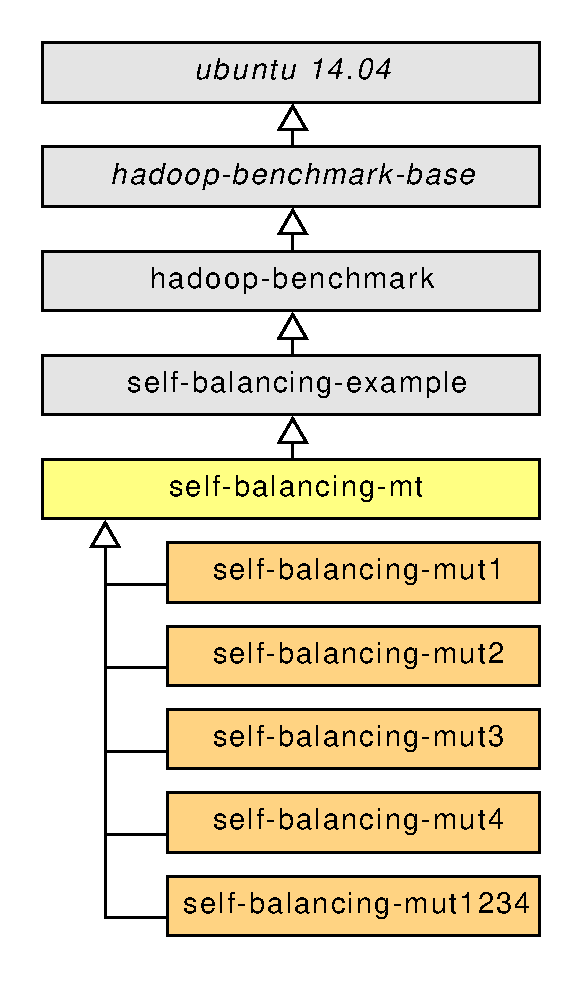
\includegraphics[width=0.4\columnwidth]
    {./resources/hadoopBenchDockerInherits.pdf}
    \caption[Vererbungshierarchie der Docker"=Images in Hadoop"=Benchmark]
    {Vererbungshierarchie der Docker"=Images in Hadoop"=Benchmark.
    Die kursiv markierten Images können nicht mithilfe von Hadoop"=Benchmark gestartet werden, die grau unterlegten Images sind in Hadoop"=Benchmark enthalten bzw. benötigt.}
    \label{fig:hadoopBenchDockerInherits}
\end{wrapfigure}

Das reale Cluster wurde mithilfe der Plattform Hadoop"=Benchmark umgesetzt.
Hierzu wurden speziell für diese Fallstudie verschiedene Szenarien entwickelt, mithilfe denen das Cluster mit den benötigten Einstellungen bzw. den zu testenden Mutanten gestartet wurde.
Um die Verwaltung des Clusters zu vereinfachen wurden zudem entsprechende Setup- und Startscripte entwickelt, die auch von den implementierten Connectoren genutzt wurden.

\subsection{Grundlegender Aufbau}
\label{subsec:clusterBasics}

Da Docker (genutzt wird hier Version 18.03 CE) und Hadoop vor allem zum Einsatz in Linux"=Umgebungen entwickelt wurden, werden für das reale Cluster bis zu zwei physische Linux"=Hosts genutzt.
Auf einem dieser beiden Hosts wird mithilfe von VirtualBox 5.2 eine VM mit Windows 10 Education Version 1803 ausgeführt, um die Tests mithilfe von \ac{ss} auszuführen.
Dies ist nötig, da \ac{ss} mithilfe des .NET"=Frameworks entwickelt wurde (vgl. \cref{sec:ssharp}), welches auf Linux zudem nur in einem verringertem Funktionsumfang verfügbar ist \cite{Schwichtenberg2017}.

Die beiden Hosts sind jeweils mit einem Intel Core i5"=4570 @ 3,2 GHz x 4, 16 GB Arbeitsspeicher sowie einer SSD ausgestattet, auf der Ubuntu 16.04 LTS als Betriebssystem installiert ist.

Insgesamt wurden für diese Fallstudie die 6 in \cref{fig:hadoopBenchDockerInherits} gelb bzw. orange hinterlegten Szenarien mit den entsprechenden Docker"=Images entwickelt.
Das zentrale Image in dieser Fallstudie ist das gelb hinterlegte \texttt{self-balancing-mt}, in dem alle benötigten angepassten Einstellungen enthalten sind.
Dies betrifft \zB die Anpassung der Zeitabstände zur Erkennung von defekten Nodes oder das Starten des \ac{TLS}, welcher in den Standard"=Szenarien der Plattform nicht gestartet wird.
Die orange hinterlegten Images dienen zur Ausführung der  Mutationstests.
Die Images enthalten daher nur die mutierte Selfbalancing"=Komponente, welche dadurch die in \texttt{self-balancing-example} enthaltene überschreiben.
Das Namenssuffix der Images bzw. Szenarien in Form der Nummern geben an, welche der in \cref{sec:implMutationTests} generierten Mutationen enthalten sind.

\subsection{HostMode des Clusters}
\label{subsec:hostMode}

Der bereits mehrfach erwähnte \texttt{HostMode} beschreibt den prinzipiellen Aufbau des gestarteten Clusters.
Es ist hierbei möglich, das Cluster wie in \cref{sec:hadoopBenchmark} beschrieben mithilfe von Docker Machine zu starten, wodurch entsprechende VMs gestartet werden, auf denen das Cluster auf Docker"=Containern ausgeführt wird.
Der größte Nachteil dieses \texttt{DockerMachine}"=Modes ist, dass das Cluster nicht bzw. nur umständlich auf mehreren Hosts ausgeführt werden kann.

Um das Cluster auf beiden für diese Fallstudie genutzten Hosts auszuführen, wurde daher der \texttt{Multihost}"=Mode entwickelt, bei dem die Docker"=Container des Clusters direkt auf den jeweiligen Hosts ohne Docker Machine gestartet werden:

\begin{figure}[h]
    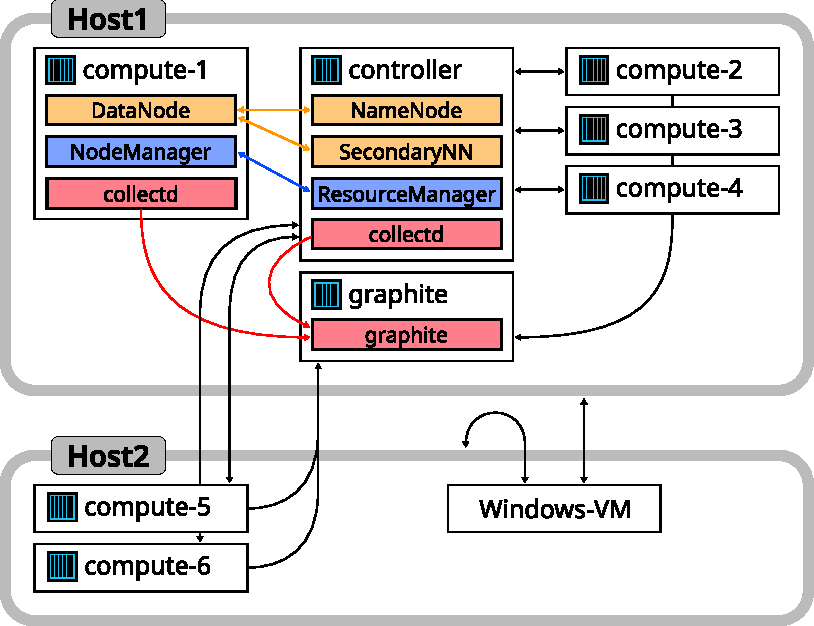
\includegraphics{./resources/caseStudyHadoopSetup.pdf}
    \caption[Cluster"=Setup bei der Nutzung des Multihost"=Modes]
    {Cluster"=Setup bei der Nutzung des \texttt{Multihost}"=Modes.
    Hier ist das konkrete, in dieser Fallstudie genutzte Setup gezeigt.
    Grün: \ac{HDFS}, Blau: \ac{YARN}, Rot: Graphite.}
    \label{fig:caseStudyHadoopSetup}
\end{figure}

Die genaue Anzahl der zu nutzenden Hosts und der Hadoop"=Nodes ist in beiden \texttt{HostMode}s variabel, wodurch es auch möglich ist, das Cluster nur auf Host1 zu starten.
Damit das Cluster jedoch auf beiden Hosts gestartet werden kann, ist es nötig, zuvor beide Hosts als Docker"=Swarm miteinander zu verbinden.
Außerdem können mithilfe des \texttt{Multihost}"=Modes dem Hadoop"=Cluster weitere, sonst für die Ausführung der VMs benötigte Ressourcen, zur Verfügung gestellt werden.

Je nach \texttt{HostMode} unterscheiden sich einzelne Pfade oder Adressen, \zB die der REST"=API.
Auch aus diesem Grund wurde die bereits in \cref{subsec:modelClass} erläuterte Klasse \texttt{ModelSettings} entwickelt, welche die Verwaltung der entsprechenden Pfade und Adressen übernimmt.

\subsection{Setup- und Startscripte}
\label{subsec:scripts}

Die Plattform Hadoop"=Benchmark enthält bereits zum Starten des Clusters ein Setup"=Script und zum Ausführen der Benchmarks entsprechende Start"=Scripte.
Um die Interaktion aufgrund der beiden unterschiedlichen \texttt{HostMode}s zu vereinfachen, wurde dennoch für jeden \texttt{HostMode} ein Setup"=Script entwickelt, um die jeweils gleiche Befehlssyntax bereitstellen zu können.
Die beiden entwickelten Setup"=Scripte werden vom \texttt{CmdConnector} genutzt um die benötigten Aktionen auf dem Cluster auszuführen (vgl. \cref{subsubsec:implCmdConnector}).
Die beiden Setup"=Scripte abstrahieren somit die vom \texttt{HostMode} abhängigen, benötigten Befehle und sorgen dafür, dass der genutzte \texttt{HostMode} transparent ist, benötigen hierfür jedoch die gleiche, in \cref{app:setupScriptCmds} gezeigte, Befehlssyntax.
Sie beinhalten entsprechende Befehle für folgende Aktionen:

\begin{itemize}
    \item Starten und Beenden des gesamten Clusters
    \item Injizieren und Reparieren von Komponentenfehlern
    \item Ausführen von \ac{CLI}"=Befehlen von Hadoop
\end{itemize}

Zudem wird beim Starten des Clusters immer geprüft, ob sich die Dockerfiles geändert haben und entsprechend die Docker"=Images aktualisiert, aus denen das Cluster gestartet wird.
Die Setup"=Scripte enthalten außerdem weitere, jeweils spezifische Befehle zum Umgang mit dem Cluster im entsprechenden \texttt{HostMode}.

Zum zentralen Starten der Benchmarks wurde ebenfalls ein zentrales Benchmark"=Startscript entwickelt, welches die jeweiligen Start"=Scripte der einzelnen Benchmarks ausführt.
Dadurch kann analog zum Setup"=Script unabhängig vom zu startenden Benchmark vom \texttt{CmdConnector} immer der gleiche Syntax genutzt werden.
Das zentrale Benchmark"=Startscript ermittelt basierend auf dem zu startenden Benchmark das jeweils benötigte Start"=Script und übergibt die jeweils benötigten Parameter.
Die vom \texttt{HostMode} abhängigen Parameter zum Starten der Benchmark"=Container werden von den hierfür angepassten Start"=Scripten der Benchmarks selbst ermittelt.
Die jeweiligen Startparameter der Anwendungen selbst werden vom Benchmark"=Controller (vgl. \cref{subsec:appImplementation}) bereitgestellt.

